\documentclass{article}
\usepackage{tikz, comment}
\usepackage{pifont}
\usepackage{fontspec}
\usetikzlibrary{arrows, decorations.markings, decorations.pathreplacing}
\begin{comment}
:Title: Not defined yet
:Tags: rose;revolution;positive;periodic;period;multiple;function
:Author: Prof.Hu Ji-shan, HKUST
:Slug: No name yet

Description Here.........
\end{comment}
\begin{document}\centering

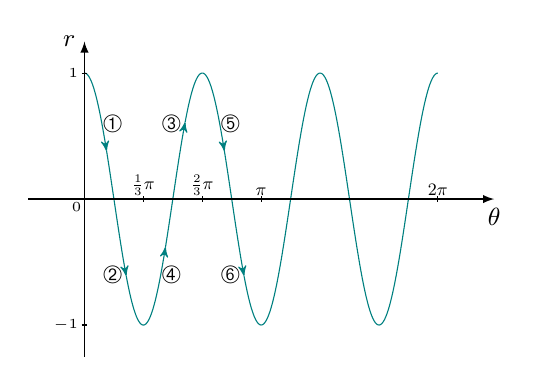
\begin{tikzpicture}[>=latex,xscale=.5/0.7, yscale=.5*3.2][font=\sf\small]

\draw[->, >=stealth', teal, samples=150, smooth, domain=0:pi/8, variable=\t]
plot ({\t}, {cos(3*\t r)}) -- ({pi/8}, {cos(3*(pi/8) r)});

\draw[->, >=stealth', teal, samples=150, smooth, domain=pi/8:pi/8+pi/9, variable=\t]
plot ({\t}, {cos(3*\t r)}) -- ({pi/8+pi/9}, {cos(3*(pi/8+pi/9) r)});

\draw[->, >=stealth', teal, samples=150, smooth, domain=pi/8+pi/9:pi/8+3*pi/9, variable=\t]
plot ({\t}, {cos(3*\t r)}) -- ({pi/8+3*pi/9}, {cos(3*(pi/8+3*pi/9) r)});

\draw[->, >=stealth', teal, samples=150, smooth, domain=pi/8+3*pi/9:pi/8+4*pi/9, variable=\t]
plot ({\t}, {cos(3*\t r)}) -- ({pi/8+4*pi/9}, {cos(3*(pi/8+4*pi/9) r)});

\draw[->, >=stealth', teal, samples=150, smooth, domain=pi/8+4*pi/9:pi/8+6*pi/9, variable=\t]
plot ({\t}, {cos(3*\t r)}) -- ({pi/8+6*pi/9}, {cos(3*(pi/8+6*pi/9) r)});

\draw[->, >=stealth', teal, samples=150, smooth, domain=pi/8+6*pi/9:pi/8+7*pi/9, variable=\t]
plot ({\t}, {cos(3*\t r)}) -- ({pi/8+7*pi/9}, {cos(3*(pi/8+7*pi/9) r)});

\draw[teal, samples=150, smooth, domain=pi/8+7*pi/9:2*pi, variable=\t]
plot ({\t}, {cos(3*\t r)});

%\draw[xstep=1cm,ystep=1cm,color=gray!80] (0, -1) grid (8, 8);
\foreach \x in {}
\draw (\x,2pt/6) -- (\x,-2pt/6)
node[anchor=north] {\tiny$\x$}
;
\draw ({1*pi/3},2pt/3.2) -- ({1*pi/3},-2pt/3.2)node[anchor=south, xshift=0, scale=0.7] {$\frac{1}{3}\pi$};
\draw ({2*pi/3},2pt/3.2) -- ({2*pi/3},-2pt/3.2)node[anchor=south, xshift=0, scale=0.7] {$\frac{2}{3}\pi$};
\draw ({pi},2pt/3.2) -- ({pi},-2pt/3.2)node[anchor= south, xshift=0, scale=0.7] {$\pi$};
\draw ({2*pi},2pt/3.2) -- ({2*pi},-2pt/3.2)node[anchor= south, xshift=0, scale=0.7] {$2\pi$};

\foreach \x in {}
\draw (\x,2pt*1.5) -- (\x,-2pt*1.5)
node[anchor=south] {\tiny$\x$}
;
\foreach \y in {-1,1}
\draw (-2pt*0.7,\y) -- (2pt*0.7,\y)
node[anchor=east] {\tiny $\y$}
;

\draw[->] (-1, 0) -- ({2*pi+1}, 0)node[below] {\small $\theta$} ;
\draw[->] (0, -1.25) -- (0, 1.25)node[left] {\small $r$} ;

\node at ({0.5}, 0.6) {\ding{192}};
\node at ({0.5}, -0.6) {\ding{193}};
\node at ({0.5+pi/3}, 0.6) {\ding{194}};
\node at ({0.5+pi/3},-0.6) {\ding{195}};
\node at ({0.5+2*pi/3}, 0.6) {\ding{196}};
\node at ({0.5+2*pi/3},-0.6) {\ding{197}};

\node at (-0.2*0.7, -0.2/3.2) {\tiny$0$};

\end{tikzpicture}\hskip0.5cm
\end{document}